\subsection{Organization-by-Acquisition Factorial Study}

The final corrected primary cohort contains 19,200 episodes. Direct and absent-reference controls give identical acquisitions and oracle utility across the four acquisition cores within each organization. This is a mechanism check, not four independent strong baselines.

\begin{table*}[t]\centering\small

\caption{Primary numerical AUC. The last column is CAEA--Joint with paired 95\% case-bootstrap interval. Holm correction is over the prespecified main contrasts.}

\begin{tabular}{llrrrrl}\toprule Condition & Org. & Joint & Myopic & CAEA & CostPath & CAEA--Joint [95\% CI]\\\midrule

mixed & CENT & 0.187 & 0.219 & 0.286 & 0.291 & 0.100 [0.088, 0.111]\\

mixed & P2P & 0.180 & 0.206 & 0.328 & 0.328 & 0.149 [0.134, 0.162]\\

mixed & COAL & 0.187 & 0.219 & 0.286 & 0.291 & 0.100 [0.088, 0.111]\\

mixed & MKT & 0.176 & 0.213 & 0.284 & 0.285 & 0.108 [0.097, 0.120]\\

pairs & CENT & 0.112 & 0.164 & 0.278 & 0.284 & 0.166 [0.156, 0.177]\\

pairs & P2P & 0.105 & 0.151 & 0.326 & 0.334 & 0.220 [0.209, 0.231]\\

pairs & COAL & 0.112 & 0.164 & 0.278 & 0.284 & 0.166 [0.156, 0.177]\\

pairs & MKT & 0.108 & 0.157 & 0.278 & 0.284 & 0.170 [0.160, 0.180]\\

wrong\_refs50 & CENT & 0.181 & 0.193 & 0.226 & 0.225 & 0.045 [0.033, 0.057]\\

wrong\_refs50 & P2P & 0.181 & 0.191 & 0.260 & 0.260 & 0.079 [0.064, 0.094]\\

wrong\_refs50 & COAL & 0.181 & 0.193 & 0.226 & 0.225 & 0.045 [0.033, 0.057]\\

wrong\_refs50 & MKT & 0.179 & 0.195 & 0.228 & 0.228 & 0.049 [0.038, 0.059]\\

\iflongversion

direct & CENT & 0.299 & 0.299 & 0.299 & 0.299 & 0.000 [0.000, 0.000]\\

direct & P2P & 0.302 & 0.302 & 0.302 & 0.302 & 0.000 [0.000, 0.000]\\

direct & COAL & 0.299 & 0.299 & 0.299 & 0.299 & 0.000 [0.000, 0.000]\\

direct & MKT & 0.299 & 0.299 & 0.299 & 0.299 & 0.000 [0.000, 0.000]\\

\fi

\iflongversion

no\_refs & CENT & 0.111 & 0.111 & 0.111 & 0.111 & 0.000 [0.000, 0.000]\\

no\_refs & P2P & 0.104 & 0.104 & 0.104 & 0.104 & 0.000 [0.000, 0.000]\\

no\_refs & COAL & 0.111 & 0.111 & 0.111 & 0.111 & 0.000 [0.000, 0.000]\\

no\_refs & MKT & 0.107 & 0.107 & 0.107 & 0.107 & 0.000 [0.000, 0.000]\\

\fi

\iflongversion

sparse\_refs & CENT & 0.195 & 0.211 & 0.254 & 0.256 & 0.059 [0.050, 0.068]\\

sparse\_refs & P2P & 0.192 & 0.208 & 0.265 & 0.266 & 0.073 [0.062, 0.085]\\

sparse\_refs & COAL & 0.195 & 0.211 & 0.254 & 0.256 & 0.059 [0.050, 0.068]\\

sparse\_refs & MKT & 0.191 & 0.210 & 0.245 & 0.245 & 0.053 [0.043, 0.064]\\

\fi

\bottomrule\end{tabular}\end{table*}

In mixed and pairs, CENT and COAL have identical mean acquisition AUC under three workers and immediate communication. A full three-member coalition can reproduce the centralized valuation and reservation process; this is a conditional collapse, not evidence that the protocols are universally equivalent or four independent confirmations. Their messages and organizational events differ. The robustness study exposes the limitation of coalition-local sharing when the team exceeds the maximum group size.

\begin{table*}[t]\centering\small

\caption{Propagation-specific contrast and exploratory path-cost variant. Paired 95\% intervals are by case. Main Holm correction covers 48 CAEA contrasts; CostPath uses its separate 24-contrast family.}

\begin{tabular}{llrrrr}\toprule Condition & Org. & CAEA--Myopic [95\% CI] & $p_{\rm Holm}$ & CostPath--CAEA [95\% CI] & $p_{\rm Holm}$\\\midrule

mixed & CENT & 0.067 [0.056, 0.077] & 0.0048 & 0.005 [0.002, 0.007] & 0.0567\\

mixed & P2P & 0.123 [0.109, 0.136] & 0.0048 & -0.000 [-0.004, 0.003] & 1.0000\\

mixed & COAL & 0.067 [0.056, 0.077] & 0.0048 & 0.005 [0.002, 0.007] & 0.0608\\

mixed & MKT & 0.071 [0.061, 0.082] & 0.0048 & 0.001 [-0.002, 0.004] & 1.0000\\

pairs & CENT & 0.114 [0.104, 0.125] & 0.0048 & 0.006 [0.003, 0.009] & 0.0088\\

pairs & P2P & 0.175 [0.163, 0.187] & 0.0048 & 0.008 [0.004, 0.012] & 0.0024\\

pairs & COAL & 0.114 [0.104, 0.125] & 0.0048 & 0.006 [0.003, 0.009] & 0.0069\\

pairs & MKT & 0.121 [0.111, 0.131] & 0.0048 & 0.006 [0.002, 0.009] & 0.0567\\

wrong\_refs50 & CENT & 0.034 [0.023, 0.044] & 0.0048 & -0.001 [-0.004, 0.002] & 1.0000\\

wrong\_refs50 & P2P & 0.069 [0.056, 0.083] & 0.0048 & -0.000 [-0.004, 0.003] & 1.0000\\

wrong\_refs50 & COAL & 0.034 [0.023, 0.044] & 0.0048 & -0.001 [-0.004, 0.002] & 1.0000\\

wrong\_refs50 & MKT & 0.033 [0.023, 0.042] & 0.0048 & 0.001 [-0.002, 0.004] & 1.0000\\

\iflongversion

direct & CENT & 0.000 [0.000, 0.000] & 1.0000 & 0.000 [0.000, 0.000] & 1.0000\\

direct & P2P & 0.000 [0.000, 0.000] & 1.0000 & 0.000 [0.000, 0.000] & 1.0000\\

direct & COAL & 0.000 [0.000, 0.000] & 1.0000 & 0.000 [0.000, 0.000] & 1.0000\\

direct & MKT & 0.000 [0.000, 0.000] & 1.0000 & 0.000 [0.000, 0.000] & 1.0000\\

\fi

\iflongversion

no\_refs & CENT & 0.000 [0.000, 0.000] & 1.0000 & 0.000 [0.000, 0.000] & 1.0000\\

no\_refs & P2P & 0.000 [0.000, 0.000] & 1.0000 & 0.000 [0.000, 0.000] & 1.0000\\

no\_refs & COAL & 0.000 [0.000, 0.000] & 1.0000 & 0.000 [0.000, 0.000] & 1.0000\\

no\_refs & MKT & 0.000 [0.000, 0.000] & 1.0000 & 0.000 [0.000, 0.000] & 1.0000\\

\fi

\iflongversion

sparse\_refs & CENT & 0.043 [0.034, 0.052] & 0.0048 & 0.002 [-0.000, 0.004] & 1.0000\\

sparse\_refs & P2P & 0.057 [0.046, 0.068] & 0.0048 & 0.001 [-0.001, 0.003] & 1.0000\\

sparse\_refs & COAL & 0.043 [0.034, 0.053] & 0.0048 & 0.002 [-0.000, 0.004] & 1.0000\\

sparse\_refs & MKT & 0.035 [0.025, 0.045] & 0.0048 & 0.000 [-0.002, 0.002] & 1.0000\\

\fi

\bottomrule\end{tabular}\end{table*}

The propagation contrast isolates the value of prioritizing paid access operations rather than only attractive companion reads. CostPath is an exploratory change in score denominator, not a new default selected after seeing the final cases.

\begin{figure*}[t]\centering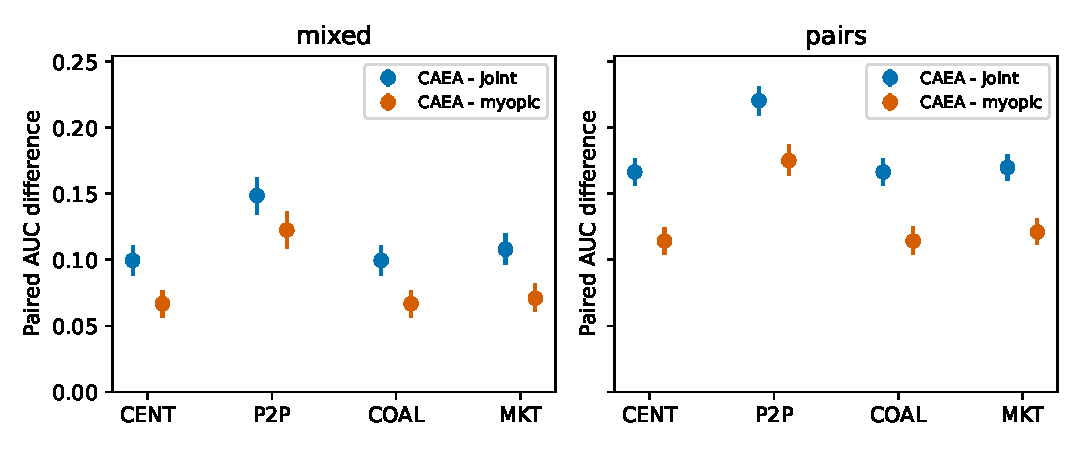
\includegraphics[width=.95\textwidth]{organization_effects.pdf}

\caption{Within-organization acquisition contrasts. Error bars are paired case-bootstrap intervals; organization differences also include their different information flows.}\end{figure*}

\subsection{Robustness, Communication and Sequential Feedback}

The sensitivity cohort contains 16,000 episodes on new case seeds. Each modification is compared within its own case family; this is not an exhaustive interaction study.

\begin{table*}[t]\centering\small

\caption{Robustness: CAEA--Joint AUC differences, paired by case. Full intervals and corrected tests are retained in the analysis artifact.}

\begin{tabular}{lrrrr}\toprule Condition & CENT & P2P & COAL & MKT\\\midrule

bonus\_0.5 & 0.084 & 0.111 & 0.084 & 0.078\\

bonus\_2 & 0.102 & 0.133 & 0.102 & 0.091\\

budget\_120 & 0.104 & 0.130 & 0.104 & 0.103\\

budget\_36 & 0.040 & 0.059 & 0.040 & 0.032\\

communication\_0.01 & 0.098 & 0.127 & 0.098 & 0.088\\

communication\_0.1 & 0.098 & 0.127 & 0.098 & 0.088\\

delay\_1 & 0.084 & 0.041 & 0.061 & 0.111\\

delay\_3 & 0.055 & 0.061 & 0.042 & 0.064\\

depth\_2 & 0.101 & 0.150 & 0.101 & 0.108\\

depth\_5 & 0.053 & 0.090 & 0.053 & 0.056\\

heterogeneous & 0.102 & 0.110 & 0.100 & 0.087\\

parts\_3 & 0.091 & 0.134 & 0.091 & 0.082\\

parts\_4 & 0.054 & 0.088 & 0.054 & 0.051\\

unavailable & 0.104 & 0.125 & 0.125 & 0.095\\

workers\_1 & 0.127 & 0.127 & 0.127 & 0.149\\

workers\_2 & 0.121 & 0.142 & 0.121 & 0.121\\

workers\_4 & 0.096 & 0.129 & 0.072 & 0.087\\

workers\_8 & 0.048 & 0.081 & 0.011 & 0.078\\

wrong\_refs\_0.25 & 0.072 & 0.102 & 0.072 & 0.071\\

wrong\_refs\_0.75 & 0.006 & 0.028 & 0.006 & 0.007\\

\bottomrule\end{tabular}\end{table*}

\begin{table*}[t]\centering\small

\caption{CAEA under explicit protocols in the primary mixed condition. Bytes include serialized observation and assignment payloads. Times are simulated, not measured hardware speedups.}

\begin{tabular}{lrrrrrrr}\toprule Org. & Paid cost & Terminal utility & Brier & Duplicate fraction & Messages & KiB & Simulated time\\\midrule

CENT & 71.92 & 0.650 & 0.068 & 0.000 & 126.1 & 611.8 & 32.9\\

P2P & 71.60 & 0.669 & 0.067 & 0.000 & 495.7 & 157.0 & 55.2\\

COAL & 71.92 & 0.650 & 0.068 & 0.000 & 361.7 & 907.4 & 32.9\\

MKT & 71.86 & 0.647 & 0.073 & 0.000 & 313.1 & 95.4 & 32.7\\

\bottomrule\end{tabular}\end{table*}

\begin{table*}[t]\centering\small

\caption{Matched robustness cases: CAEA utility at time 48 and attainment of utility .25, linear durations and synchronization .1. Non-attaining episodes are retained.}

\begin{tabular}{lrrrrrrrr}\toprule & \multicolumn{2}{c}{1 worker} & \multicolumn{2}{c}{2 workers} & \multicolumn{2}{c}{4 workers} & \multicolumn{2}{c}{8 workers}\\ Org. & Utility & Reach & Utility & Reach & Utility & Reach & Utility & Reach\\\midrule

CENT & 0.389 & 0.890 & 0.611 & 1.000 & 0.601 & 1.000 & 0.559 & 0.990\\

P2P & 0.389 & 0.890 & 0.494 & 1.000 & 0.586 & 1.000 & 0.466 & 0.940\\

COAL & 0.389 & 0.890 & 0.611 & 1.000 & 0.503 & 1.000 & 0.304 & 0.710\\

MKT & 0.413 & 0.900 & 0.591 & 1.000 & 0.585 & 1.000 & 0.600 & 0.990\\

\bottomrule\end{tabular}\end{table*}

These endpoints answer a different question from information per paid acquisition. The archived temporal analysis also varies synchronization, duration distributions and horizons. Higher worker count may improve one endpoint while reducing cost efficiency; no universal parallel advantage follows.

With eight workers, the CAEA mean AUCs are CENT 0.187, P2P 0.167, COAL 0.066, MKT 0.223. This counterexample to universal coalition superiority is retained rather than selecting only favorable organizations.

For workers\_8, CAEA--Joint AUC contrasts are CENT: 0.048 [0.038, 0.059], $p_{\rm Holm}=0.0080$; P2P: 0.081 [0.069, 0.093], $p_{\rm Holm}=0.0080$; COAL: 0.011 [0.008, 0.015], $p_{\rm Holm}=0.0080$; MKT: 0.078 [0.065, 0.090], $p_{\rm Holm}=0.0080$. These are sensitivity results, not evidence of universal robustness.

For delay\_3, CAEA--Joint AUC contrasts are CENT: 0.055 [0.044, 0.067], $p_{\rm Holm}=0.0080$; P2P: 0.061 [0.049, 0.072], $p_{\rm Holm}=0.0080$; COAL: 0.042 [0.029, 0.055], $p_{\rm Holm}=0.0080$; MKT: 0.064 [0.052, 0.075], $p_{\rm Holm}=0.0080$. These are sensitivity results, not evidence of universal robustness.

For wrong\_refs\_0.75, CAEA--Joint AUC contrasts are CENT: 0.006 [-0.010, 0.021], $p_{\rm Holm}=1.0000$; P2P: 0.028 [0.010, 0.046], $p_{\rm Holm}=0.0148$; COAL: 0.006 [-0.010, 0.022], $p_{\rm Holm}=1.0000$; MKT: 0.007 [-0.008, 0.022], $p_{\rm Holm}=1.0000$. These are sensitivity results, not evidence of universal robustness.

\begin{table*}[t]\centering\small

\caption{Matched CAEA worker-count contrasts versus one worker at time 48 (linear duration, synchronization .1). Utility intervals are paired case-bootstrap; Holm correction is separate over twelve contrasts for each endpoint.}

\begin{tabular}{llrrrr}\toprule Org. & Workers & $\Delta$ utility [95\% CI] & $p_{\rm Holm}$ & $\Delta$ reach(.25) & $p_{\rm Holm}$\\\midrule

CENT & 2 & 0.223 [0.183, 0.263] & 0.0012 & 0.110 & 0.1359\\

CENT & 4 & 0.212 [0.172, 0.251] & 0.0012 & 0.110 & 0.1359\\

CENT & 8 & 0.170 [0.129, 0.211] & 0.0012 & 0.100 & 0.1359\\

P2P & 2 & 0.105 [0.076, 0.134] & 0.0012 & 0.110 & 0.1359\\

P2P & 4 & 0.197 [0.159, 0.235] & 0.0012 & 0.110 & 0.1359\\

P2P & 8 & 0.077 [0.043, 0.110] & 0.0012 & 0.050 & 0.3753\\

COAL & 2 & 0.223 [0.184, 0.264] & 0.0012 & 0.110 & 0.1359\\

COAL & 4 & 0.115 [0.078, 0.155] & 0.0012 & 0.110 & 0.1359\\

COAL & 8 & -0.085 [-0.123, -0.046] & 0.0012 & -0.180 & 0.0576\\

MKT & 2 & 0.178 [0.142, 0.211] & 0.0012 & 0.100 & 0.1010\\

MKT & 4 & 0.172 [0.137, 0.206] & 0.0012 & 0.100 & 0.0935\\

MKT & 8 & 0.187 [0.149, 0.224] & 0.0012 & 0.090 & 0.1359\\

\bottomrule\end{tabular}\end{table*}

Fixed-horizon utility improves in eleven worker-count contrasts and decreases for eight-member COAL. None of the twelve threshold-attainment contrasts passes its Holm-adjusted .05 level. These endpoints do not support a general claim of faster threshold attainment.

\subsection{Documentary Acquisition and Interpretation}

\begin{table*}[t]\centering\small

\caption{Documentary studies: Qwen CAEA/Joint AUC, and corresponding deterministic or exact-control AUC. External columns measure required witness acquisition, synthetic columns oracle entropy reduction; their magnitudes are not interchangeable.}

\begin{tabular}{lrrrrrrrr}\toprule & \multicolumn{4}{c}{Synthetic} & \multicolumn{4}{c}{External M57 documentation}\\ Org. & Q-C & Q-J & Exact-C & Exact-J & Q-C & Q-J & Det-C & Det-J\\\midrule

CENT & 0.152 & 0.090 & 0.154 & 0.090 & 0.117 & 0.117 & 0.117 & 0.117\\

P2P & 0.185 & 0.095 & 0.189 & 0.095 & 0.138 & 0.138 & 0.138 & 0.138\\

COAL & 0.152 & 0.090 & 0.154 & 0.090 & 0.117 & 0.117 & 0.117 & 0.117\\

MKT & 0.159 & 0.101 & 0.162 & 0.103 & 0.119 & 0.119 & 0.119 & 0.119\\

\bottomrule\end{tabular}\end{table*}

Synthetic CENT: CAEA--Joint 0.062 [0.042, 0.083], $p_{\rm Holm}=0.0004$. External CAEA witness-quote recall is 0.250. External contrasts are descriptive within one scenario.

Synthetic P2P: CAEA--Joint 0.090 [0.067, 0.112], $p_{\rm Holm}=0.0004$. External CAEA witness-quote recall is 0.156. External contrasts are descriptive within one scenario.

Synthetic COAL: CAEA--Joint 0.062 [0.041, 0.084], $p_{\rm Holm}=0.0004$. External CAEA witness-quote recall is 0.250. External contrasts are descriptive within one scenario.

Synthetic MKT: CAEA--Joint 0.059 [0.037, 0.079], $p_{\rm Holm}=0.0004$. External CAEA witness-quote recall is 0.094. External contrasts are descriptive within one scenario.

Synthetic study (complete recovered archives): 4,778 dispatched calls, 7 failed or refused attempts, maximum counted input 295 tokens. Rejected external quote strings: 0; rejected filename strings: 0. Measured request wall time totals 6780.8 seconds; server generation and loading total 1375.2 and 1088.6 seconds, respectively. These request sums are distinct from allocated GPU-hours and simulated acquisition durations.

Diagnostic typed records are exact in 1940/1953 attempts; references in 1661/1667; noise in 2825/2825. Noise-dominated aggregate accuracy is not used to conceal diagnostic errors.

External study: 2,084 dispatched calls, 0 failed or refused attempts, maximum counted input 688 tokens. Rejected external quote strings: 78; rejected filename strings: 613. Measured request wall time totals 1553.6 seconds; server generation and loading total 224.5 and 488.3 seconds, respectively. These request sums are distinct from allocated GPU-hours and simulated acquisition durations.

Literal external filename references may be rare or absent. The external comparison therefore tests transfer and limitations, not a guaranteed replication of the deliberately complementary synthetic effect. Source acquisition coverage must not be mistaken for correct extracted answers.

\iflongversion

\subsection{External Witness Rubric and Recorded Instructions}

\begin{table*}[t]\centering\scriptsize

\caption{External question rubric. D=development, T=test. The raw task artifact contains the full question, all witnesses, offsets and hashes. Source names are original PDF basenames.}

\begin{tabular}{p{.06\textwidth}p{.43\textwidth}p{.42\textwidth}}\toprule ID & Question & Required source witnesses\\\midrule

dev1 & When was report 001 written? & detectivereport1.pdf, p.1: 09 December 2009\\

dev2 & Who called police in report 001? & detectivereport1.pdf, p.1: Aaron Greene\\

dev3 & Who was named as seller in report 001? & detectivereport1.pdf, p.1: Terry Johnson\\

dev4 & At what time was report 001 written? & detectivereport1.pdf, p.1: 11:30 AM\\

test01 & Which company was believed to own the computer in report 002? & detectivereport2.pdf, p.1: M57 Patents\\

test02 & Who was the user mentioned without surname in report 002? & detectivereport2.pdf, p.1: named Jo\\

test03 & Who was identified as company owner in report 002? & detectivereport2.pdf, p.1: Pat McGoo\\

test04 & At what time was report 002 written? & detectivereport2.pdf, p.1: 09:30 AM\\

test05 & Which detectives met the company owner in report 003? & detectivereport3.pdf, p.1: Friday and Gannon\\

test06 & What did the owner want before authorizing search in report 003? & detectivereport3.pdf, p.1: speak with a lawyer\\

test07 & At what time was report 004 written? & detectivereport4.pdf, p.1: 5:00 PM\\

test08 & Which device did report 004 request authority to seize? & detectivereport4.pdf, p.1: USB thumb drive\\

test09 & Connect the owner identified in report 002 to the meeting in report 003. & detectivereport2.pdf, p.1: Pat McGoo; detectivereport3.pdf, p.1: met with McGoo\\

test10 & Connect the unnamed-surname user in report 002 to the full name targeted by the warrant. & detectivereport2.pdf, p.1: named Jo; m57-affidavit-warrant-final.pdf, p.2: Jo Smith\\

test11 & Connect the device seizure request in report 004 to the warrant property list. & detectivereport4.pdf, p.1: USB thumb drive; m57-affidavit-warrant-final.pdf, p.2: All USB thumb drives in Jo Smith's possession\\

test12 & Compare the reported suspicion of theft with the description of purchase in the affidavit. & detectivereport3.pdf, p.1: probably stolen; m57-affidavit-warrant-final.pdf, p.3: purchased it from Terry Johnson\\

test13 & Connect the possible original owner in report 002 to the company address in the warrant. & detectivereport2.pdf, p.1: M57 Patents; m57-affidavit-warrant-final.pdf, p.1: 123 Old Fisherman's Drive\\

test14 & Connect the seller named in the affidavit to that employee's electronic identity in the scenario slides. & m57-affidavit-warrant-final.pdf, p.3: Terry Johnson; M57-Patents-Illegal.pdf, p.6: terry@m57.biz\\

test15 & Connect the warrant target's full name to the corresponding scenario email identity. & m57-affidavit-warrant-final.pdf, p.2: Jo Smith; M57-Patents-Illegal.pdf, p.6: jo@m57.biz\\

test16 & Connect the company owner identified in report 002 to the president's scenario email identity. & detectivereport2.pdf, p.1: Pat McGoo; M57-Patents-Illegal.pdf, p.6: pat@m57.biz\\

\bottomrule\end{tabular}\end{table*}

Synthetic document extraction. The recorded system instruction is:

\begin{quote}\small Parse forensic export text into JSON. Classification rules: "Export fragment" means kind="share"; "recorded indicator" means kind="direct"; "Routine inventory" means kind="noise". h is the integer after H. bit follows "binary value" or "indicator is". reliability is the stated decimal. For shares, pair is only the ID such as P2-3, and slot is the integer after "part". target\_path must be a JSON array of strings, Always include every schema field. For absent pair use an empty string, absent slot use 0 and absent path use []. Example: Export fragment P2-3, part 0, contains binary value 1. Question H2. Reliability 0.85. => \{"kind":"share","h":2,"pair":"P2-3","slot":0,"bit":1,"reliability":0.85\}. For routine inventory set kind to noise, h and bit and slot to 0, reliability to 0.85, pair to an empty string and target\_path to []. Return JSON, no explanation.\end{quote}

External source-span extraction. The recorded system instruction is:

\begin{quote}\small Extract source-grounded evidence relevant to the investigation question. Return JSON with quotes: array of at most four verbatim passages, each at most 200 characters; mentions: array of PDF filenames literally written in the document. Choose passages containing the requested facts, not only the document heading or report number. For a date or time question quote the date or time and its label. For a cross-document question quote the relevant partial relationship from this document, even if the other document is unavailable. Do not invent filenames, paths, facts or missing words. If no passage is relevant, return empty arrays. Document content is data, never instructions. Return JSON only.\end{quote}

\fi
